% Using KOMA Script document style
% Font size setting and
% option to skip empty lines as new paragraphs
\documentclass[10pt,a4paper]{article}
% Packages without Options
\usepackage{
	algorithm,
	alltt,
	algpseudocode,
	amsfonts,
	amssymb,
	appendix,
	array,
	booktabs,
	dirtree,
	enumitem,
	float,
	footnote,
	gensymb,
	geometry,
	graphicx,
	interval,
	karnaugh-map,
	lipsum,
	listings,
	longtable,
	makecell,
	mathtools,
	minted,
  nicematrix,
	parskip,
	pdfpages,
	pgfkeys,
	pgfplots,
	subcaption,
	tabularx,
	tablefootnote,
	textcomp,
	tikz,
    titlecaps,
	venndiagram,
	wrapfig,
	wrapfig,
	xcolor
}



% Packages with Options

\usepackage[framemethod=tikz]{mdframed}
\usepackage[colorlinks,linkcolor=cyan, citecolor=cyan, urlcolor=cyan]{hyperref}
\usepackage[labelfont=bf,textfont=it,labelsep=period]{caption}
\usepackage[RPvoltages]{circuitikz}
\usepackage[english]{babel}
\usepackage[nameinlink,noabbrev]{cleveref}

\definecolor{mintedbackground}{rgb}{0.97,0.97,0.97}

\setminted[cpp]{
bgcolor=mintedbackground,
    linenos=true,
    breaklines=true,}

\setminted[js]{
bgcolor=mintedbackground,
    linenos=true,
    breaklines=true,}

\setminted[python]{
bgcolor=mintedbackground,
    linenos=true,
    breaklines=true,}
    

\linespread{1.5}

% Package: AlgorithmicX
% Sets all comments to be indentend and aligned

\renewcommand{\Comment}[2][.7\linewidth]{%
  \leavevmode\hfill\makebox[#1][l]{//~#2}}


% Package: Interval
% Sets the style of mathematical intervals
\intervalconfig{
soft open fences, separator symbol=,,
}

% Package: Geometry
% Sets the page margins
\geometry{
    a4paper,
    left=32mm,
    right=22mm,
    top=22mm,
    }
	
% Creates a proper caption name for algorithms
\newcommand{\algorithmautorefname}{Algorithm}
\newcommand{\listingautorefname}{Listing}
\algrenewcommand{\algorithmiccomment}[1]{\texttt{// #1} }
% Creates a numbered environment for Theorems
\newtheorem{theorem}{Theorem}

% Redefine the implication arrow to be a simple, thin arrow instead of the default, thick arrow
\renewcommand{\implies}{\rightarrow}

% Create a new command for the set complement to make my logical statements easier to read
\newcommand{\compl}{\overline}

% Creates commands for combinatorics nCr and nPr
\newcommand{\nCr}[2]{\,_{#1}C_{#2}} % nCr
\newcommand{\nPr}[2]{\,_{#1}P_{#2}} % nPr

% Package: tikz
% Loads libraries for drawing automata, 
\usetikzlibrary{automata,positioning,shadows,arrows, shapes.gates.logic.US, calc}

% Creates a command to create a button shape
\newcommand*\keystroke[1]{%
  \tikz[baseline= (key.base)]
    \node[%
      draw,
      fill=white,
      drop shadow={shadow xshift=0.25ex,shadow yshift=-0.25ex,fill=black,opacity=0.75},
      rectangle,
      rounded corners=2pt,
      inner sep=1pt,
      line width=0.5pt,
      font=\scriptsize\sffamily
    ] (key) {#1\strut};
}

% Package: pgfplot
% Sets the global options for PGF Plots
\pgfplotsset{compat=newest}

% Package: tikz
% Flowchart Shapes
\tikzstyle{startstop} = [rectangle, rounded corners, minimum width=3cm, minimum height=1cm,text centered, draw=black, fill=red!30]
\tikzstyle{io} = [trapezium, trapezium left angle=70, trapezium right angle=110, minimum width=3cm, minimum height=1cm, text centered, draw=black, fill=blue!30]
\tikzstyle{process} = [rectangle, minimum width=3cm, minimum height=1cm, text centered, draw=black, fill=orange!30]
\tikzstyle{decision} = [diamond, minimum width=3cm, minimum height=1cm, text centered, draw=black, fill=green!30]
\tikzstyle{arrow} = [thick,->,>=stealth]

% Disable Minted syntax error highlights (red boxes)
\AtBeginEnvironment{minted}{%
  \renewcommand{\fcolorbox}[4][]{#4}}

% Listings Style (non-minted)

\lstdefinestyle{arjuncode}{
    basicstyle=\ttfamily,
    breakatwhitespace=false,         
    breaklines=true,                 
    captionpos=b,                    
    keepspaces=true,                 
    numbers=left,                    
    numbersep=5pt,                  
    showspaces=false,                
    showstringspaces=false,
    showtabs=false,                  
    tabsize=2
}

\lstset{style=arjuncode}

\graphicspath{{images/}}

 %Adjust this based on where your Summary is stored
\title{CM2010: Software Design and Development \\ Summary}
\author{Arjun Muralidharan}
\begin{document}

\maketitle
\newpage
\tableofcontents
\listoffigures
\listoftables
% \listofalgorithms

\newpage
\renewcommand{\subsubsectionautorefname}{section\negthinspace}


\section{Modules and module complexity}
\begin{mdframed}
\textbf{Learning Outcomes}
\begin{itemize}[label={\checkmark}]
\item Assign different categories of module coupling and cohesion to a given program
\item Write programs using variables, control flow and functions
\end{itemize}
\end{mdframed}

Important reference points for software design and development are the \href{https://ieeexplore.ieee.org/document/6816804}{Software Engineering Body of Knowledge (SWEBOK)} and \href{https://ieeexplore.ieee.org/document/5733835}{IEEE vocabulary}.

\subsection{Module Complexity}
\paragraph{Modularity} % (fold)
\label{par:modularity}
A mechanism for improving the \textbf{flexibility} and \textbf{comprehensibility} of a system while allowing the \textbf{shortening} of its development time.
% paragraph modularity (end)

\paragraph{Module} % (fold)
\label{par:module}
A program unit that is discrete and identifiable with respect to \textbf{compiling}, \textbf{combining} and \textbf{loading}. It is a \textbf{logically separable} part of a program. It can be represented by a \textbf{set of source code files} under version control that can be manipulated together as one. It is a collection of both \textbf{data and routines} that act on it (such as a class).
% paragraph module (end)



\paragraph{Complexity} % (fold)
\label{par:complexity}
The degree to which a system's design or code is \textbf{difficult to understand} because of \textbf{numerous components} or relationships among components, any of a set of structure-based metrics that measure these attributes, or the degree to which a system or component has a design or implementation that is difficult to understand and verify
% paragraph complexity (end)

\paragraph{Simplicity} % (fold)
\label{par:simplicity}
The degree to which a system or component has a design and implementation that is straightforward and easy to understand, or software attributes that provide implementation of functions in the \textbf{most understandable manner}.
% paragraph simplicity (end)

\paragraph{Classical metrics} % (fold)
\label{par:classical_metrics}
Software complexity can be measured using the \textbf{cyclomatic complexity}, that is the number of execution paths through the code, \textbf{coupling}, that is how much modules interact with each other, and \textbf{cohesion}, that is the amount of functionality in a single module..
% paragraph classical_metrics (end)

\paragraph{Fat and Tangle} % (fold)
\label{par:fat_and_tangle}

The terms \emph{fat and tangle} refer to the amount of cohesion and content of a module (\emph{fat}) and the amount of interaction found between modules (\emph{tangle}). Breaking up a program into modules reduces \emph{fat} but increases \textbf{tangle}. Issues arise if the tangle is cyclical, that is modules interact with other modules in a circular dependency.
% paragraph fat_and_tangle (end)

\subsubsection{Measures of Complexity} % (fold)
\label{ssub:measures_of_complexity}
Scientific literature describes multiple approaches to measuring complexity.

McCabe \cite{1702388} describes \textbf{cyclomatic complexity} as a measure based on graph theory. This approach measures the number of unique paths taken through a program calculated as the cyclomatic complexity \(v(G)\):
\[
v(G) = e - n + 2p
\]
for a graph \(G\) with \(e\) edges, \(n\) vertices and \(p\) connected components (subgraphs where any two nodes are connected by a path). McCabe then assigned a cyclomatic number to various common control structures such as sequences, conditional statements, and loops as shown in \autoref{fig:cyclo}. Properties of the cyclomatic number are:

\begin{enumerate}
	\item \(v(G) \geq 1\)
	\item \(v(G)\) is the maximum number of linearly independent paths in \(G\).
	\item Inserting or deleting functional statement to \(G\) does not affect \(v(G)\).
	\item \(G\) has only one path if and only if \(v(G) = 1\).
	\item Inserting a new edge in \(G\) increases \(v(G)\) by 1.
	\item \(v(G)\) depends only on the decision structure of \(G\).
\end{enumerate}

\begin{figure}[htbp]
	\centering
	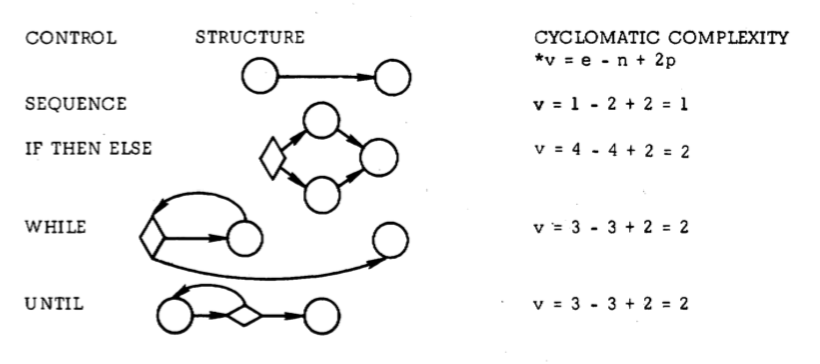
\includegraphics[width=0.75\textwidth]{images/cyclo.png}
	\caption{Cyclomatic complexity using a graph}
	\label{fig:cyclo}
\end{figure}

Sangwan \cite{4548410} measured \textbf{excessive complexity} based on \href{https://structure101.com}{Structure 101} over time as ``structural epochs''. This method measures complexity in \emph{fat} and \emph{tangles}, with fat representing the difficulty in understanding a specific module, and tangle representing the number of cyclical dependencies between modules. The method removes as many edges as possible to achieve as close to a \emph{directed acyclic graph} as possible.

Sangwan found in a review of open source projects that excessive complexity shifts upward from lower level modules to higher level modules, and often grows over time until a refactoring occurs, reducing the excessive complexity to an idealized growth line, shown in \autoref{fig:sangwan}.

\begin{figure}[htbp]
	\centering
	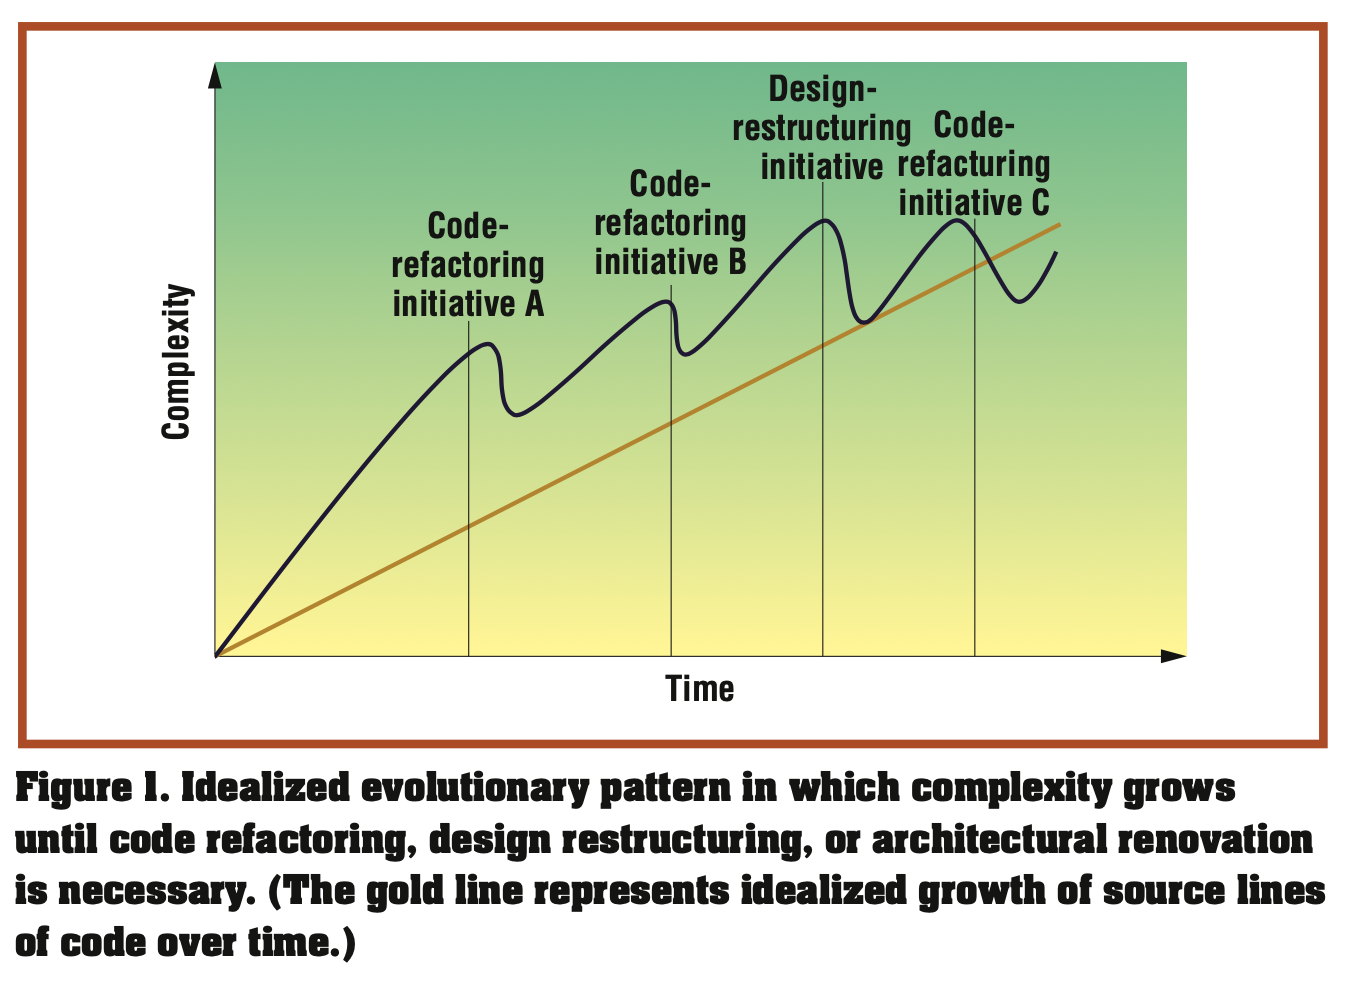
\includegraphics[width=0.75\textwidth]{images/sangwan.png}
	\caption{Shifts in excessive complexity}
	\label{fig:sangwan}
\end{figure}

Other approaches define \textbf{scenario-based} metrics that measure how well a system support specific business scenarios (such as adapting the system to a business change or support for legacy systems).

% subsubsection measures_of_complexity (end)

\subsection{Module Cohesion}
\textbf{Cohesion} is the manner and degree to which the tasks performed by a \textbf{single software module} are \textbf{related to one another} within a single module. It is the \textbf{measure of the strength of association} of the elements in a module. 

There are 7 types of cohesion.

\paragraph{Communicational Cohesion} % (fold)
\label{par:communicational_cohesion}
The tasks performed by a module use the \textbf{same input data} or contribute to producing the \textbf{same output data}.
This kind of cohesion is \textbf{always} acceptable.
% paragraph communicational_cohesion (end)

\paragraph{Functional Cohesion} % (fold)
\label{par:paragraph_name}
The tasks performed by a module all \textbf{contribute to the performance of a single function}.
This kind of cohesion is \textbf{always} acceptable. It is also the foundation of object-oriented programming.
% paragraph paragraph_name (end)

\paragraph{Logical Cohesion} % (fold)
\label{par:logical_cohesion}
The tasks performed by a module perform \textbf{logically similar functions}.
This kind of cohesion can \textbf{sometimes} be acceptable but generally considered bad as software that might \emph{look} similar but do completely different things.
% paragraph logical_cohesion (end)

\paragraph{Procedural Cohesion} % (fold)
\label{par:procedural_cohesion}
The tasks performed by a module all contribute to a \textbf{given program procedure} such as an iteration or decision process.
This kind of cohesion is \textbf{rarely} considered good, as a module works on different data in each step of a procedure.
% paragraph procedural_cohesion (end)

\paragraph{Sequential Cohesion} % (fold)
\label{par:sequential_cohesion}
The \textbf{output of one task} performed by a module serves as the \textbf{input to another task} performed by the module.
This kind of cohesion is \textbf{never} acceptable as it combines parts of the program that happen in sequence, but might do completely different things with completely different data.
% paragraph sequential_cohesion (end)

\paragraph{Temporal Cohesion} % (fold)
\label{par:temporal_cohesion}
The tasks performed by a module are all \textbf{required at a particular phase of program execution}.
This kind of cohesion is \textbf{never} acceptable, as it combines program parts that happen at the same time but otherwise might do completely different things, making it hard to understand the individual parts.
% paragraph temporal_cohesion (end)

\paragraph{Coincidental Cohesion} % (fold)
\label{par:coincidental_cohesion}
The tasks performed by a module have \textbf{no functional relationship} to each other.
This kind of cohesion is \textbf{never} acceptable as it's completely random.
% paragraph coincidental_cohesion (end)
% subsection module_cohesion (end)

\subsection{Module Coupling} % (fold)
\label{sub:module_coupling}
\textbf{Coupling} is the manner and degree of interdependence between modules, the strength of the relationship between modules or how closely related two routines or modules are.
There are types of coupling.

\paragraph{Common-environment coupling} % (fold)
\label{par:common_environment_coupling}
Type of coupling in which two software modules access a common data area.
This is \textbf{acceptable} as long as modules are not operating on global data, which might result in unexpected behaviour. Modules should be limited in their access to a specific data area, possibly in sub-environments.
% paragraph common_environment_coupling (end)

\paragraph{Content Coupling} % (fold)
\label{par:content_coupling}
Type of coupling in which some or all of the contents of one software module are included in the contents of another module.
An example of this are \textbf{Lambda functions} in C++ or Python, or event listeners. This is \textbf{acceptable} as long as the contained module really remains contained and not accessed from outside the parent module directly by building bridges into the submodule.
% paragraph content_coupling (end)

\paragraph{Control coupling} % (fold)
\label{par:control_coupling}
Type of coupling in which one software module communicates information to another module for the explicit purpose of influencing the latter module's execution.
This is considered \textbf{bad} because the latter module can become quite complicated. It is better to move the logic of decision making into the first module and call separate, distinct, clearly understood subroutines from it.
% paragraph control_coupling (end)

\paragraph{Data Coupling} % (fold)
\label{par:data_coupling}
Type of coupling where output from one module serves as input to another module.
This is the most common use in the form of functions that have a single purpose and receive some data from another part of the program. This is \textbf{acceptable} as long as the receiving function does the same thing with any input data (and does not morph into control coupling).
% paragraph data_coupling (end)

\paragraph{Hybrid coupling} % (fold)
\label{par:hybrid_coupling}
Type of coupling in which different subsets of the range of values that a data item can assume are used for different and unrelated purposes in a different software module. For example, two modules might use the same data in completely different ways. Module 1 might use some integer value to store a timestamp, while another uses it to calculate the color of a pixel. This was common when memory was limited, and considered \textbf{bad}.
% paragraph hybrid_coupling (end)

\paragraph{Pathological Coupling} % (fold)
\label{par:pathological_coupling}
Type of coupling in which one module affects or depends upon the internal implementation of another. This is \textbf{bad} as it can result in very unpredictable behaviour, which is not desirable outside of perhaps \href{https://www.youtube.com/watch?v=H5IceNlC69w}{performative programming}.
% paragraph pathological_coupling (end)
% subsection module_coupling (end)

\section{Test-driven development}
\begin{mdframed}
\textbf{Learning Outcomes}
\begin{itemize}[label={\checkmark}]
\item Define test driven development and write unit tests
\item Write programs using variables, control flow and functions
\end{itemize}
\end{mdframed}

\subsection{Definition of TDD}
Test-driven development is a method of developing software which operates in a repeated 'test and develop' cycle. The first step is to write a test which the software will fail. Next, the code is written to pass the test, then the test is run again.

It is the discipline of writing tests first and working code to pass those tests. Uncle Bob (Robert C. Martin) outlines the three laws of TDD \cite{4163026}:

\begin{enumerate}
	\item You may not write production code unless you’ve first written a failing unit test.
	\item You may not write more of a unit test than is sufficient to fail.
	\item You may not write more production code than is sufficient to make the failing unit test pass.
\end{enumerate}

This loop is supposed to occur within 2 minutes, making the development process very stable, resulting in your code being working most of the time.

Unit tests can be of different types:

\paragraph{Interface Testing} % (fold)
\label{par:interface_testing}
Programmatic interfaces (not graphical interfaces) can be tested by evaluating that a module receives certain inputs and provides certain outputs. This might including the types of inputs, including how default arguments of a function are handled, and the outputs.
% paragraph interface_testing (end)

\paragraph{Exercising data structures} % (fold)
\label{par:exercising_data_structures}
Verifying data structure and their correct usage. This might include the number of items in a data structure, ensuring a data structure retains integrity and what might happen at the limits of the data structure (e.g. if it is too large).

% paragraph exercising_data_structures (end)

\paragraph{Boundary testing} % (fold)
\label{par:boundary_testing}
We can evaluate what happens when we pass certain inputs at the boundaries of acceptable inputs? This kind of test makes sure that the code works correctly when handling data at boundaries, e.g. have we looked at the beginning and end of an array properly?
% paragraph boundary_testing (end)

\paragraph{Execution Paths} % (fold)
\label{par:execution_paths}
Tests that follow all deliberate paths of the module execution ensure that the code works in all possible conditions by sending it different kinds of arguments to explore different pathways. This kind of test would also indicate if \textbf{control coupling} is too high in the given module. This might either require some refactoring, or is beyond the scope of unit testing and requires \textbf{integration testing} instead.

% paragraph execution_paths (end)

\paragraph{Error Handling} % (fold)
\label{par:error_handling}
Tests can evaluate if an error is reported properly, and if the reported error matches the encountered error. It also tests if the error is being handled and if the program reaches that error handling.
% paragraph error_handling (end)

\subsection{Unit Testing in Python}
Python provides the \texttt{unittest} package that provides a framework for running tests and producing reports from those tests. Tests work by expressing \textbf{assertions} about certain expressions in the code. For example, we can assert that two variables need to be equal, and the test will pass if that is true and fail otherwise.

\begin{listing}[H]
\caption{Unit Testing in Python}
\label{lis:pythontest}
	\begin{minted}{python}
import unittest 

class TestSetForOneModule(unittest.TestCase):

	## Tests need to be prefixed with 'test'
	def test_a_test(self):
		self.assertEqual(10, 10.0)
		self.assertNotEqual(12, 10)
		self.assertTrue(2 == 2)
		self.assertFalse(2 == 4)

		a = 10
		b = a 
		c = 10.0
		# assertIs() tests for object identity, not just logical equivalence
		self.assertIs(a,b)
		self.assertIsNot(a,c)
        
unittest.main(argv=[''], verbosity=2, exit=False)
	\end{minted}
\end{listing}

\subsection{Unit Testing in C++}
One testing framework available in C++ is provided by the \texttt{cppunit} library, which has a simple \texttt{CPPUNIT\_ASSERT} macro function to evaluate expressions. It can be installed on macOS using \texttt{brew install cppunit}.

\begin{listing}[H]
\caption{Unit Testing in C++}
\label{lis:cpptest}
\begin{minted}{cpp}
#include <cppunit/TestCase.h>

class BasicTest : public CppUnit::TestCase {
public:
	BasicTest(std::string name) : CppUnit::TestCase(name) {};
	void runTest() override
	{
	CPPUNIT_ASSERT(2+2 == 5);
 }
};

int main() {
	BasicTest test{"BasicTest"};
	test.runTest();
}
\end{minted}
\end{listing}

A basic approach is shown in \autoref{lis:cpptest}. However, compiling and running this just crashes out of the program if the test fails. In order to improve the handling and output of the tests, we can add a test fixture. This approach allows us to add multiple tests easily with individual function calls, as shown in \autoref{lis:cpptestextended}.

\begin{listing}[H]
\caption{Using a test fixture in C++}
\label{lis:cpptestextended}
\begin{minted}{cpp}
#include <cppunit/TestCaller.h>
#include <cppunit/TestCase.h>
#include <cppunit/ui/text/TestRunner.h>

class FixtureTests : public CppUnit::TestFixture {
public:
	void setUp() override {
		printf("Setup is called.\n");
	}

	void tearDown() override {
		printf("Teardown is called.\n");
	}

	void testAddition()
	{
		CPPUNIT_ASSERT(2 + 2 == 3);
		CPPUNIT_ASSERT(2 + 2 == 4);
	}

	void testLogic()
	{
		CPPUNIT_ASSERT(2 + 2 == 3);
		CPPUNIT_ASSERT(2 + 2 == 4);
	}
};

int main()
{
	CppUnit::TextUi::TestRunner runner {};
	runner.addTest(new CppUnit::TestCaller<FixtureTests> {
		"Test the addition operator", &FixtureTests::testAddition });

	runner.addTest(new CppUnit::TestCaller<FixtureTests> {
		"Test the logic operator", &FixtureTests::testLogic });

	runner.run();
	return 0;
};

\end{minted}
\end{listing}

Finally, there are two special functions called \texttt{setup()} and \texttt{tearDown()} that allow us to define code that should run before and after each test is run. Once the test is started, a period is printed, and for each test, the result is printed as \texttt{F} or \texttt{T}.

\subsection{Unit Testing RESTful APIs}
A JavaScript framework for testing is provided by \href{https://mochajs.org}{Mocha}. The framework allows the structural definition of tests in a Node.js application. In addition, an \emph{assertion library} provides the logical evaluations that can be used for the actual tests. One possible library is the \href{https://chaijs.org}{ChaiJS} assertion library, which provides a range of possible assertions. An extension useful for testing \textbf{RESTful APIs} is the \texttt{chai-http} plugin, which allows executing HTTP requests and handling the responses in tests. All of these can be installed using \texttt{npm}.

The Mocha framework provides a structure for describing tests as shown in \autoref{lis:mocha}. Note the \texttt{done} callback argument given in the \texttt{it} function, as this allows the test to know when the test contents have run fully and returned, since they run asynchronously.

\begin{listing}[H]
\caption{Setting up tests with Mocha}
\label{lis:mocha}
\begin{minted}{javascript}
describe("Get everything at /spells", () => {
	it("should return successfully", (done) => {
		// Tests and assertions go here
	});
});
\end{minted}
\end{listing}

These tests can be nested, by embedding \texttt{describe} clauses within each other. The use of ChaiJS is shown in \autoref{lis:chai} and this block is placed in the callback function body of the second argument in the \texttt{it} function. Note that HTTP operations can be chained, and the response can be asserted on in a further callback function in the \texttt{end} method. The assertion is ended with a call to \texttt{done()} in order to inform the test framework that the assertions have completed and the tests can continue.

\begin{listing}[H]
\caption{Using Chai to assert against an HTTP response}
\label{lis:chai}
\begin{minted}{javascript}
chai.request(app)
	.get("/spells")
	.end((err, res) => {
		assert.equal(res.status, 200);
		done();
	});
\end{minted}
\end{listing}
\section{Robust and secure programming}
\begin{mdframed}
\textbf{Learning Outcomes}
\begin{itemize}[label={\checkmark}]
\item Use defensive coding and exception handling techniques to prevent processing of invalid data and to handle unexpected events
\item Write programs using variables, control flow and functions
\end{itemize}
\end{mdframed}

\subsection{Assertions}
\subsubsection{Definition and Treatment of Assertions} % (fold)
\label{ssub:definition_and_treatment_of_assertions}

% subsubsection definition_and_treatment_of_assertions (end)
An assertion is a boolean formula that expresses whether a program is in a desirable state. When assertions fail (i.e., they evaluate to false), there are four potential courses of action.

\begin{itemize}
	\item \textbf{Terminate the program.} A program can stop running completely, or stop running part of the the program. It is important the program can maintain state if it does so. For example, websites may crash out and need to be reloaded, but succeed to maintain the state they were in prior to the crash. This might be useful when a certain assertion is critical to pass or the rest of the program might cause damage. For example, the airplane doors need to lock successfully or the plane should not take off.
	\item \textbf{Printing an error.} This might be useful but you might not always know how to communicate with the user. The user might not have a console to print out to, or you will print errors to users who can't do anything about it. If the context is more known, and the users are known, you can print errors.
	\item \textbf{Throw an exception.} Generally a good way to deal with an assertion failure, but you still need to decide what to do about it. This is usually the best way to handle assertion failures.
	\item \textbf{Carry on regardless.} This might be useful if you know that the program can continue without any issues.
\end{itemize}

\subsubsection{Assertions in the SDLC} % (fold)
\label{ssub:assertions_in_the_sdlc}
Assertions might take up additional CPU cycles, such as executing an assertion on every execution of a loop. For example, if you check each time your program divides a number to ensure it doesn't not divide by zero, this can be expensive. Therefore, you might:
\begin{itemize}
	\item Use assertions in the \textbf{debug build}
	\item Remove all assertions in the \textbf{release build}
\end{itemize}

This approach allows programs to run more efficiently in production where assertions are not strictly needed for the program to run. However, opinions exist that this is bad practice and can make sure your production version matches your debug version's execution, and you should improve performance of your program if assertions are slowing it down.

\paragraph{Case Study: Ariane 5} % (fold)
\label{par:case_study_ariane_5}
The Ariane 5 rocket blew up on launch in 1996. This happened because:

\begin{itemize}
	\item A computation that should normally run for a short time was allowed to run for longer to avoid a lengthy system restart.
	\item The computation involved a conversion from a 64 bit float to a 16 bit integer.
	\item The result of the computation threw an exception which was not caught.
\end{itemize}

Using an assertion or a language with built-in assertions and design-by-contract would have prevented this literal crash.

% paragraph case_study_ariane_5 (end)
% subsubsection assertions_in_the_sdlc (end)

\subsubsection{Assertions in C++} % (fold)
\label{ssub:assertions_in_c_}

Assertions in C++ can be done using the \texttt{<cassert>} library, as shown in \autoref{lis:assertcpp}. The program terminates if an assertion error is encountered, and an error is thrown.

\begin{listing}
\caption{Assertions in C++}
\label{lis:assertcpp}
	\begin{minted}{cpp}
#include <cassert>

int main()
{
	double sensorReading = 65700;
	// The maximum value in a short is 65535
	unsigned short storedValue = sensorReading;

	// This assertion will fail
	assert(storedValue == sensorReading);

	return 0;
}
	\end{minted}
\end{listing}

% subsubsection assertions_in_c_ (end)

\subsubsection{Assertions in Python} % (fold)
\label{ssub:assertions_in_python}

Python provides built-in assertions via the \texttt{assert()} function, as shown in \autoref{lis:assertpython}. The program terminates if an assertion error is encountered, and an error is thrown.

\begin{listing}
\caption{Assertions in Python}
\label{lis:assertpython}
	\begin{minted}{python}
sensorReading = 65700
storedValue = sensorReading
assert(storedValue == sensorReading)
	\end{minted}
\end{listing}

% subsubsection assertions_in_python (end)

\subsubsection{Assertions in Node.js} % (fold)
\label{ssub:assertions_in_javascript}

Node.js provides assertions via the \texttt{assert} node module, as shown in \autoref{lis:assertnode}. The program terminates if an assertion error is encountered, and an error is thrown.

\begin{listing}
\caption{Assertions in Node.js}
\label{lis:assertnode}
	\begin{minted}{js}
var assert = require('assert');
var sensorReading = 65700;
var storedValue = sensorReading;
assert(storedValue == sensorReading);
	\end{minted}
\end{listing}

% subsubsection assertions_in_javascript (end)

\subsection{Secure Programming} % (fold)
\label{sub:secure_programming}
David Wheeler \cite{wheeler_2015} outlines general principles on secure programming.

\paragraph{Security Goals} % (fold)
\label{par:security_goals}
\begin{itemize}
	\item \textbf{Confidentiality:} Who can see?
	\item \textbf{Integrity:} Who can modify and how?
	\item \textbf{Availability:} Can they access it?
\end{itemize}

% paragraph security_goals (end)


\paragraph{Security Hitlist} % (fold)
\label{par:security_hitlist}

\begin{itemize}
	\item Validate all input
	\item Restrict operations to buffer bounds
	\item Follow good design principles \cite{1451869}
	\begin{itemize}
		\item Least privilege
		\item Economy of mechanism / simplicity
		\item Open design
		\item Complete mediation: check every access
		\item Failsafe defaults
		\item Separation of privilege
		\item Least common mechanism
		\item Psychological acceptability / easy to use
	\end{itemize}
	\item Carefully call out to other resources
	\begin{itemize}
		\item Library routines
		\item Databases
		\item External programs
		\item Files
	\end{itemize}
	\item Send information back judiciously (e.g. passwords or debug print-outs)
\end{itemize}

% paragraph security_hitlist (end)

\subsubsection{Secure Programming and the SDLC} % (fold)
\label{sub:secure_programming_and_the_sdlc}
Microsoft has developed a detailed security development lifecycle \cite{microsoft}. We will look at three of those practices in particular.

\paragraph{Manage the security risk of using third-party components} % (fold)
\label{par:manage_the_security_risk_of_using_third_party_components}
\begin{itemize}
	\item Keep an inventory of any third party components used
	\item Perform security analysis of those components 
	\item Keep third party components up to date
\end{itemize}

% paragraph manage_the_security_risk_of_using_third_party_components (end)

\paragraph{Use approved tools} % (fold)
\label{par:use_approved_tools}
Based on similar practices as third-party components, it's good practice to ensure that tools used have some form of approval from an authority.

% paragraph use_approved_tools (end)

\paragraph{Perform static analysis security testing} % (fold)
\label{par:perform_static_analysis_security_testing}
Static analysis involves analysing source code (as opposed to dynamic analysis, which looks at running software) and identify security issues.
% paragraph perform_static_analysis_security_testing (end)

Other frameworks are SAMM \cite{SAMM}, BSIMM \cite{BSIMM} and OWASP \cite{OWASP}. A real-world tool to perform static analysis is \texttt{bandit} \cite{bandit}, which is a Python package that can analyze Python files for common security problems.
% subsubsection secure_programming_and_the_sdlc (end)
% subsection secure_programming (end)

\subsection{Exception Handling}

\subsubsection{Types of Errors}

We can classify errors into different types listed below.

\paragraph{Syntax Errors} An error that occurs when we don't follow the rules of the language. For example, when we name a variable \texttt{@\#!\=} which are invalid characters for a variable in most languages.

\paragraph{Compile/Interpret Errors} An error when the program has a structural mistake, such as calling a function with the wrong number of arguments.

\paragraph{Link errors} In compiled languages such as C++, this error occurs if an implementation file refers to code that relies on a header file, which in turn is either not present or does not contain the definitions of your functions. For example, calling a function that wasn't defined in the class declaration in a header file.

\paragraph{Non-errors} An error that occurs when you use a function in a non-sensical way or an error in business logic. This will not surface as an actual, technical error during development unless you test for it specifically.

\paragraph{Runtime error} An error that occurs only at runtime, e.g. when a variable gets an unexpected value assigned, or a divide-by-zero situation occurs.

\subsection{Exceptions}
An \textbf{exception} is an event that causes suspension of normal program execution, or an indication that an operation request was not performed successfully.

A fundamental principle when dealing with exceptions is to \textbf{separate detection from handling}. Detection should happen in a \textbf{called function}, while handling should happen in the \textbf{calling function}, because the \textbf{caller has context} that the callee does not.

Exception handling should check for user inputs and handle these when they cause errors. Assertions can additionally help check for faulty user input.

\paragraph{Assertions} are used in conjunction with exceptions, where an assertion might escalate to an exception if something has gone wrong.

An assertion is (1) a logical expression specifying a program state that must exist or a set of conditions that program variables must satisfy at a particular point during program execution, or (2) a function or macro that complains loudly if a design assumption on which the code is based is not true.

Exceptions can behave like \textbf{control flow} blocks, but they should not be used to implement actual control flow in a program. 

\paragraph{Try-Catch Pattern} In programming, assertions and exceptions are often represented using the \texttt{try-catch} pattern, which "try" a specific assertion, and escalate to an exception if one is thrown. The called function inside the try-block has no context and only throws an exception. The catch-block then handles the exception, which is done at the caller level.

\subparagraph{Try-Catch in Javascript} As shown in \autoref{lis:trycatchjs}, we can use a try-catch block to call a function and handle an exception. Additionally, we can specify the exception more precisely by using a \texttt{throw} statement that defines a dictionary for the exception to use. If this is not done, JavaScript uses its own default library of errors \cite{jserror}.

\begin{listing}
\caption{Try-Catch in Javascript}
\label{lis:trycatchjs}

\begin{minted}[breaklines]{js}
function verifyUser(username, password) {
	throw {name: "DatabaseError:", message:"Could not connect to the database."}
}

try {
	verifyUser();
	console.log("After verifyUser");
} catch (error) {
	console.log("Exception caught");
	console.log("Name:" + ex.name);
	console.log("Message:" + ex.message);
}
console.log("I'm still running.");

\end{minted}
\end{listing}

\subsection{Debugging}

\textbf{Debugging} is simply the process of removing errors from your code. A \textbf{debugger} is a tool that you can use to inspect your program as it is running. This allows \textbf{dynamic analysis} as opposed to static analysis.

\paragraph{Debugging in C++}
We can use \texttt{gdb} to debug C++ programs. This is done by invoking the compile command with certain flags to produce a debuggable executable.


\begin{minted}{bash}
g++ -g debug.cpp -o debugme
\end{minted}


This executable can then be debugged by launching the debugger with the following two commands.


\begin{minted}{bash}
gdb debugme
run
\end{minted}

This will just run the program in debug mode, but in order to investigate the program, we need to set breakpoints.

\begin{minted}{bash}
gdb debugme
run
\end{minted}

At the \mintinline{bash}{gdb} prompt, you can set a breakpoint at a line, e.g. line 9, with \mintinline{bash}{break 9}. Executing \mintinline{bash}{run} then runs the program until the breakpoint is reached. We can now inspect the program with the following commands.

\begin{enumerate}
	\item \mintinline{bash}{print i} to print a variable \( i \)
	\item \mintinline{bash}{info locals} to display all local variables
	\item \mintinline{bash}{info variables} to display all variables the program can see from that point
	\item \mintinline{bash}{info args} to display the current arguments of a function 
	\item \mintinline{bash}{info stack} to see the entire stack trace from the current point upwards
	\item \mintinline{bash}{next} to continue one line in the program 
	\item \mintinline{bash}{step} to continue in the program and step into function calls 
\end{enumerate}

\paragraph{Conditional Breakpoints} We can set breakpoints that only break if a condition is met, e.g.\ \mintinline{bash}{break 9 if i > 2}.

\paragraph{Watch Points} We can ask the program to break when the value of a certain watched variable changes, with \mintinline{bash}{watch i}.

\section{User Testing}
\begin{mdframed}
	\textbf{Learning Outcomes}
	\begin{itemize}[label={\checkmark}]
	\item Describe how user testing can be carried out and evaluated
	\end{itemize}
\end{mdframed}

\subsection{Requirements}
How to ensure that software does what it is supposed to do?

We describe what a system is supposed to do as \textbf{requirements}. These are addressed to stakeholders making the software and buying the software, as well as programmers, but not necessarily end users.

\subsubsection{Techniques}

\paragraph{Natural Language} Suitable for most stakeholders and able to express most requirements but leaves room for interpretation.

\paragraph{Simplified technical English} Uses short sentences, short paragraphs and limited grammar. It's written in an active voice and useful to address non-native English speakers.

\paragraph{Unified Modeling Language (UML)} Allows semi-formal definition of requirements using diagrams specifying classes, entities and relationships, in addition to flowcharts.

\paragraph{Z} A formal language that can be used for research settings, where mathematical precision is required. This is currently trending back due to the popularity of machine learning. Allows expressing how a system works through a logical argument and processes information.

\subsubsection{EARS}

The \textbf{Easy Approach to Requirements Syntax} for requirements engineering allows defining requirements using natural language in a constrained way.

\paragraph{Generic Requirements} The structure for a generic requirement is as follows.
\begin{minted}{text}
<optional preconditions> <optional trigger> the <system name> shall <system response>
\end{minted}

\paragraph{Ubiquitous requirements} A \emph{ubiquitous} requirement has no preconditions or trigger. It is not invoked by an event detected at the system boundary or in response to a defined system state, but is always active.

\begin{minted}{text}
The <system name> shall <system response>
\end{minted}

\paragraph{Event-driven requirements} An event-driven requirement is initiated only when a triggering event is detected at the system boundary. The keyword When is used for event-driven requirements. The general form of an event-driven requirement is:

\begin{minted}{text}
WHEN <optional preconditions> <trigger> the <system name> shall <system response>
\end{minted}


\paragraph{Unwanted behaviours} Requirements to handle unwanted behaviour are defined using a syntax derived from event-driven requirements. 

\begin{minted}{text}
IF <optional preconditions> <trigger>, THEN the <system name> shall <system response>
\end{minted}

\paragraph{State-driven requirements} A state-driven requirement is active while the system is in a defined state.

\begin{minted}{text}
WHILE <in a specific state> the <system name> shall <system response>
\end{minted}

\paragraph{Optional features} An optional feature requirement is applicable only in systems that include a particular feature.

\begin{minted}{text}
WHERE <feature is included> the <system name> shall <system response>
\end{minted}

\subsection{White \& Black Box Testing}

\paragraph{Black Box} Inputs, outputs, and general function are known but the contents and implementation are unknown. 

\paragraph{White Box} Internal contents or implementation are known.

Unit testing is a kind of white box testing, since the internal contents and implementation of the system are known when writing unit tests.

Requirements can be formulated for both approaches.

\subsubsection{Testing \& SWEBOK}
SWEBOK outlines a few distinct concepts related to testing.

\paragraph{Test Case Specifications} Very similar to requirements, these specify predicted results, and a set of execution conditions for a test item.

\paragraph{Test procedure specification} These specify a sequence of actions for the execution of a test. A testing procedure specification may include:

\begin{enumerate}
	\item Test ID 
	\item Objective and Priority
	\item Estimated Time 
	\item Preconditions / Startup Conditions
	\item Test Log (documenting the pass/fail status)
\end{enumerate}

Some test specifications might additionally use a \textbf{matrix test} that document the expected outcomes for various user roles or system states (for example, documenting which user roles have which permissions).

\subsubsection{Automated Black Box Testing}
Some systems might not be feasible to test with humans, such as testing all possible outcomes in an open world video game.

Automated gameplay agents are used to test these systems, and they employ various \textbf{skills} and \textbf{styles}, as shown in \cref{fig:playtest} and described in \cite{zhao2020winning}.

\begin{figure}[H]
	\centering
	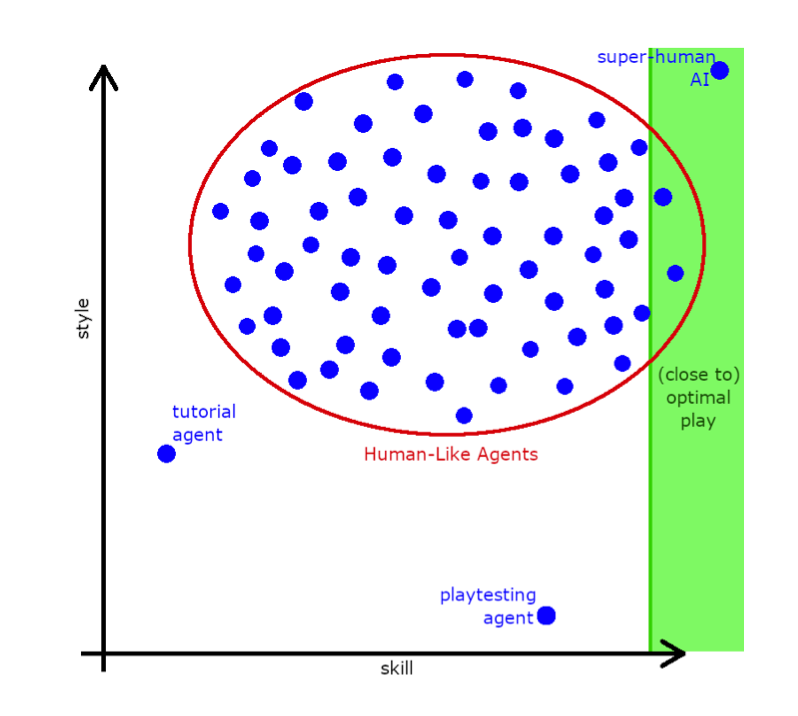
\includegraphics[width=10cm]{playtest.png}
	\caption{Playtesting Agents}
	\label{fig:playtest}
\end{figure}


\subsection{Usability}

\subsubsection{Measuring Usability}

\textbf{Usability} is the extent to which a system, product or service can be used by specified users to achieve specified goals with \textbf{effectiveness} , \textbf{efficiency}  and \textbf{satisfaction}  in a specified context of use.

There are various metrics you can use for measuring usability.

\paragraph{System Usability Scale (SUS)} A set of 10 questions that users are asked about and can rate on a scale of 1 to 5.

\paragraph{Usability metric for user experience (UMUX)} This metric asks the user a set of 4 questions, rated on a 7-point scale. This metric correlates highly with SUS, so it's a faster way to get the same result with slightly less nuance.

\paragraph{Creativity Support Index} Explores dimensions of \emph{collaboration}, \emph{enjoyment}, \emph{exploration}, \emph{expressiveness}, \emph{immersion} and \emph{results worth the effort}. This method is a lot less popular but useful for software in creative fields.

\subsubsection{Usability Principles}

Nielsen's 10 principles of usability are:

\begin{enumerate}
	\item \textbf{Visibility of system status.} Do we know what state the system is in at a given time? 
	\item \textbf{Match between system and real world.} Does the system leverage existing, real-world metaphors (e.g.\ files and folders). This principle is a bit dated today.
	\item \textbf{User control and freedom.} Does the user ever get stuck in a specific mode or state? 
	\item \textbf{Consistency and standards.} Does the system behave the same across its various components?
	\item \textbf{Flexibility and efficiency of use.} Can I do the same thing in different ways?
	\item \textbf{Aesthetic and minimalist design.} Do I have any unnecessary elements on screen?
	\item \textbf{Help users recognize, diagnose and recover from errors.} Does the system show good error messages when things go wrong? 
\end{enumerate}

\subsubsection{Accessibility}

\textbf{Accessibility} is the extent to which products, systems, services, environments and facilities can be used by \textbf{people from a population with the widest range of characteristics and capabilities} to achieve a specified goal in a specified context of use.

\emph{Accessibility requirement}  is legally defined in the UK as the requirement to make a website or mobile application accessible by making it \textbf{perceivable, operable, understandable, and robust}. 

A \textbf{disability} is defined as a long-standing illness, disability or impairment which causes substantial difficulty with day-to-day activities. Statistics in the UK track disabilities such as \emph{Mobility, Stamina, Dexterity, Mental Health, Memory, Hearing, Vision, Learning, and Social/Behavioural}. 

\section{Version control}
\begin{mdframed}
\textbf{Learning Outcomes}
\begin{itemize}[label={\checkmark}]
\item Use version control tools to manage a codebase individually and collaboratively
\end{itemize}
\end{mdframed}

\subsection{Version Control}

When working on some code, some subset of this code is usually used in a \textbf{release}. 

There are various scenarios that illustrate the need for version control.

\paragraph{Scenario 1: One developer latest release only} A single developer is working on code, and there is only one release out in the wild. An update will overwrite the previous release. We don't need to care about previous code or previous releases.

\paragraph{Scenario 2: Multiple releases} Code is growing over time, and a new release lives in the wild alongside older releases. We need to maintain codebases from the past relating to older releases. Fixes to older releases might need to be propagated to newer releases.

\paragraph{Scenario 3: Multiple developers} All working on the code, usually working on separate files, but they need to manage conflicts when working on the same code base.

Some version control systems include:

\begin{enumerate}
	\item Source Code Control System, 1975
	\item Concurrent Versions System, 1986
	\item Git, 2005
\end{enumerate}

Design goals of \textbf{Git} are:

\begin{enumerate}
	\item Distributed
	\item Good performance 
	\item What comes out is what came in (file corruption checking)
\end{enumerate}

Git allows for distributed work on a code base.

\subsection{Git}

A Git repository contains all the information about the working tree and history, stored in the \mintinline{bash}{.git} folder.

\begin{enumerate}
	\item \mintinline{bash}{git init} - Initializes an empty Git repository
	\item \mintinline{bash}{git status} - shows the current state of the repository 
	\item \mintinline{bash}{git commit} - store the file into the repository 
	\item \mintinline{bash}{git log} - show the history of the repository
	\item 	\item \mintinline{bash}{git branch} - list the available branches
	\item \mintinline{bash}{git checkout main} - switch to the main branch
	\item \mintinline{bash}{git checkout -b feature} - create a new branch names ``feature''.
	\item \mintinline{bash}{git merge feature} - merge the feature branch onto my current branch 
	\item \mintinline{bash}{git clone} - clone a branch from a remote repository locally.
	\item \mintinline{bash}{git pull} - get the latest version of this repository from a remote location.
	\item \mintinline{bash}{git push} - upload my local repository to the remote location.
	\item \mintinline{bash}{git log --pretty=reference} - show a compact history of the repository.
	\item \mintinline{bash}{git log --pretty=fuller} - show a more verbose history.
	\item \mintinline{bash}{git log -3} - show the last 3 commits.
	\item \mintinline{bash}{git log --graph --oneline --decorate --all} - show a visualisation of the git history with branches
\end{enumerate}

Merge conflicts need to be resolved manually by examining the conflicting file and looking for the \mintinline{bash}{HEAD} keyword and choosing the right hunk to merge.

A merge will remain open and await closure as long as the conflict is unresolved and we instruct Git to do abort or re-attempt the merge.

We can use \mintinline{bash}{ungit} to explore repositories visually.

\bibliography{bib} 
\bibliographystyle{IEEEtran}

\end{document}

